\chapter{Numerical Experiments}
In this chapter, we will solve the eigenvalue problem, Eq.(\ref{eq:eigenvalue-problem}), with different discretizations. There will be three major categories of methods used. Finite difference (FD) method, finite element (FE) method and spectral element method (SE).

The finite difference method will be used together with equally spaced nodes. The finite element method will use B-spline as basis functions. Finally, the spectral element method uses sine functions as the spectral elements.

For Dirichlet boundary, The parameters of different discretizations are listed below
\begin{table} [H]
	\centering
	\caption{With Dirichlet boundary condition, all methods have good accuracy, so using 101 nodes in the region $[0,1]$ is enough. For FE and SE methods, they are using ~50 basis functions.}
	\begin{tabular}{|c|c|c|c|}
		\hline
		& FD & FE\_BSPLINE & SE\_SINE  \\
		\hline
		N & 101 & 101 & 101 \\
		\hline
		NUM\_BASIS &  & 51 & 50 \\
		\hline
	\end{tabular}
	\label{table:parameters-dirichlet}
\end{table}

For left-fixed and right-open (fixed-open) boundary condition, the parameters are    
\begin{table} [H]
	\centering
	\caption{With fixed-open boundary condition, it requires higher resolution in order to get accurate results. Therefore all methods use 501 nodes in the region $[0,1]$, and FE method uses 101 basis functions.}
	\begin{tabular}{|c|c|c|}
		\hline
		& FD & FE\_BSPLINE \\
		\hline
		N & 501 & 501 \\
		\hline
		NUM\_BASIS &  & 101 \\
		\hline
	\end{tabular}
	\label{table:parameters-fixed-open}
\end{table}


\section{Constant Velocity Case}
\subsection{Dirichlet Boundary}
Because the existence of exact solution to problems Eq.(\ref{eq:constant-v-problem-dirichlet}). The case with constant velocity profile is used as a sanity check. It allows us to verify the correctness of each method's implementation. This also serves as a reference to the accuracy spectral methods can achieve.

From Fig.(\ref{fig:constant-v}), we see that the order of growth rates obtained by different methods is about $~10^{-14}$ for both subsonic and supersonic cases. We will use these numbers as a reference to the accuracy of our numerical methods. If a method produces growth rates with order close to $10^{-14}$, we consider the growth rates to be 0.

\begin{table} [H]
	\centering
	\caption{Relative error of each eigenvalue.}
	\begin{tabular}{|c|c|c|c|c|c|}
		\hline
		$v_0=0.5$   & 1 & 2 & 3 & 4 & 5 \\
		\hline
		FD & 2.827e-05 & 1.130e-04 & 2.541e-04 & 4.512e-04 & 7.040e-04 \\
		\hline
		FE & 0.005 & 0.005 & 0.006 & 0.008 & 0.010  \\
		\hline
		SE & 2.896e-05 & 1.157e-04 & 2.603e-04 & 4.626e-04 & 7.217e-04 \\
		\hline
	\end{tabular}
	\begin{tabular}{|c|c|c|c|c|c|}
		\hline
		$v_0=1.5$   & 1 & 2 & 3 & 4 & 5 \\
		\hline
		FD & 0.001 & 0.005 & 0.010 & 0.019 & 0.030 \\
		\hline
		FE & 0.006 & 0.010 & 0.019 & 0.029 & 0.043  \\
		\hline
		SE & 0.001 & 0.005 & 0.011 & 0.019 & 0.030 \\
		\hline
	\end{tabular}
	\label{table:eigenvalue-error-dirichlet}
\end{table}

\begin{figure}[H]
	\centering
	\begin{subfigure}{0.5\textwidth}
		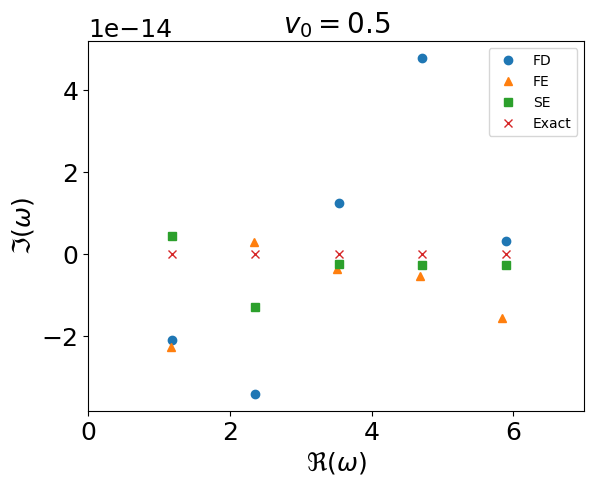
\includegraphics[width=\linewidth]{../../thesis/img/numerical-experiments/fixed-fixed/constant-v-v0=0.5}
		\caption{All modes are stable.}
	\end{subfigure}%
	\begin{subfigure}{0.5\textwidth}
		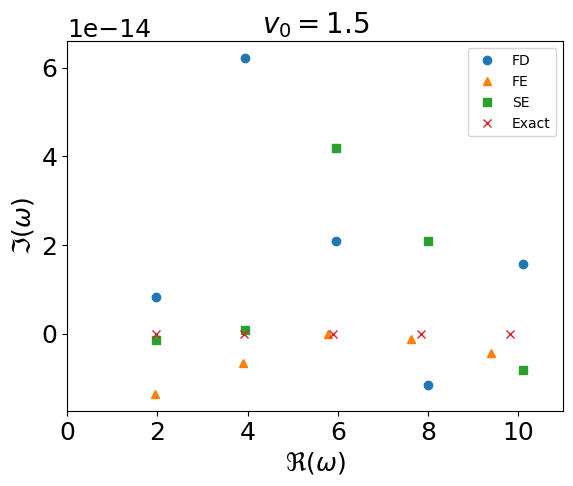
\includegraphics[width=\linewidth]{../../thesis/img/numerical-experiments/fixed-fixed/constant-v-v0=1.5}
		\caption{Filtered modes are stable.}
	\end{subfigure}
	\caption{Showing the first 5 eigenvalues of each method in each case. All methods are close to the exact eigenvalues.}
	\label{fig:constant-v-dirichlet}
\end{figure}

\subsection{Fixed-Open Boundary}
\begin{table} [H]
	\centering
	\caption{Relative error of each eigenvalue. Notice that the ground mode for subsonic case is non-zero.}
	\begin{tabular}{|c|c|c|c|c|c|}
		\hline
		$v_0=0.5$   & 0 & 1 & 2 & 3 & 4 \\
		\hline
		FD & 1.209e-05 & 3.458e-05 & 5.775e-05 & 8.153e-05 & 1.061e-04 \\
		\hline
		FE & 8.090e-05 & 2.007e-04 & 2.981e-04 & 6.596e-04 & 1.821e-03  \\
		\hline
	\end{tabular}
	\begin{tabular}{|c|c|c|c|c|c|}
		\hline
		$v_0=1.5$   & 1 & 2 & 3 & 4 & 5 \\
		\hline
		FD & 9.163e-05 & 2.435e-04 & 4.833e-04 & 8.160e-04 & 1.243e-03 \\
		\hline
		FE & 4.431e-04 & 7.924e-04 & 1.516e-03 & 3.103e-03 & 8.001e-03  \\
		\hline
	\end{tabular}
	\label{table:eigenvalue-error}
\end{table}

\begin{figure}[H]
	\centering
	\begin{subfigure}{0.5\textwidth}
		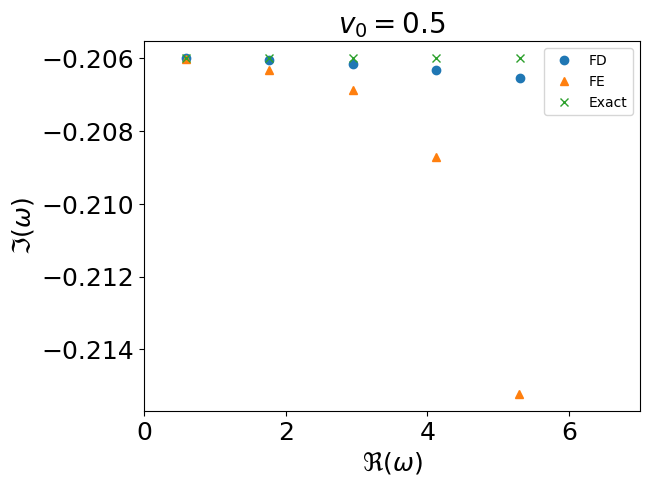
\includegraphics[width=\linewidth]{../../thesis/img/numerical-experiments/fixed-open/constant-v-v0=0.5}
		\caption{All modes are stable.}
	\end{subfigure}%
	\begin{subfigure}{0.5\textwidth}
		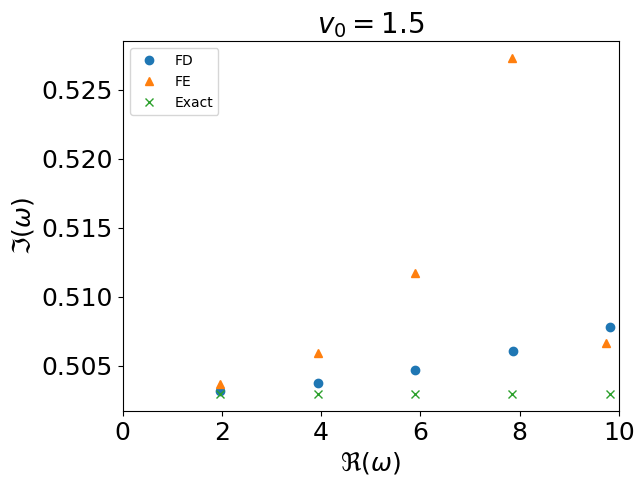
\includegraphics[width=\linewidth]{../../thesis/img/numerical-experiments/fixed-open/constant-v-v0=1.5}
		\caption{All modes are unstable.}
	\end{subfigure}
	\caption{Showing the first 5 eigenvalues of each method. Finite-difference method has much better accuracy than finite-element method.}
	\label{fig:constant-v-fixed-open}
\end{figure}


\section{Subsonic Case}
\subsection{Dirichlet Boundary}
When setting the mid-point velocity to be $M_m=0.5$, we have the subsonic velocity profile. This velocity profile is the orange line shown in Fig.\ref{fig:velocity-profiles}. With Dirichlet boundary condition, $\tilde{v}(\pm 1) =0$. The flow in magnetic nozzle is stable. Fig.\ref{fig:subsonic-v-dirichlet} shows the first few eigenvalues obtained by different discretizations. 

The order of growth rates obtained by different methods is $10^{-13}$, we can consider it to be stable.
\begin{figure} [H]
	\centering
	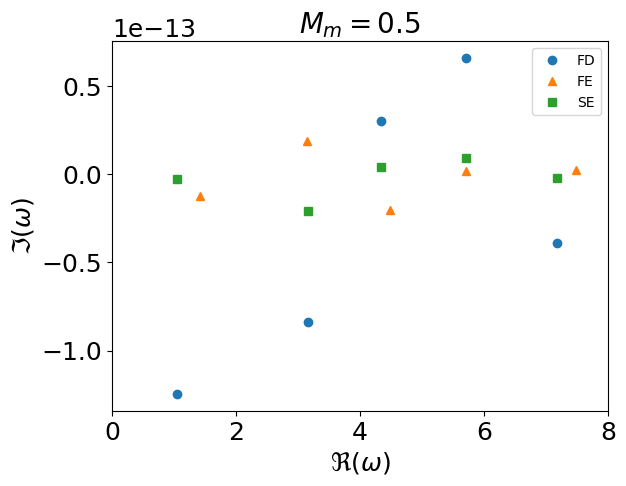
\includegraphics[width=0.7\linewidth]{../../thesis/img/numerical-experiments/fixed-fixed/subsonic-v}
	\caption{Showing the first 5 modes. It suggests that the flow in magnetic nozzle with subsonic velocity profile and Dirichlet boundary condition is stable.}
	\label{fig:subsonic-v-dirichlet}
\end{figure}

\subsection{Fixed-Open Boundary}
\begin{figure} [H]
	\centering
	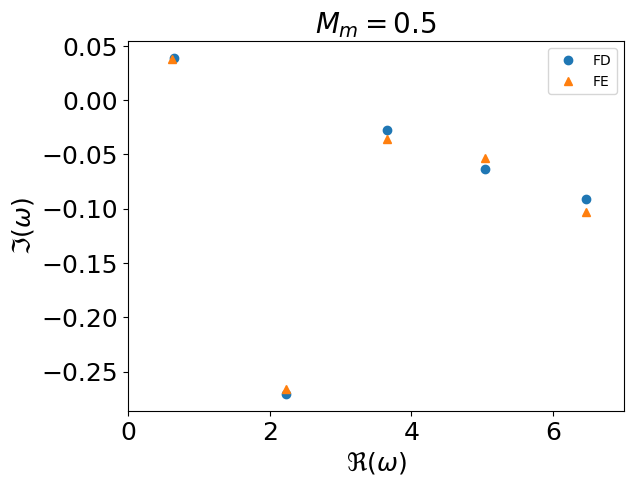
\includegraphics[width=0.7\linewidth]{../../thesis/img/numerical-experiments/fixed-open/subsonic-v}
	\caption{Showing the first 5 modes. The ground mode is unstable, other modes are stable.}
	\label{fig:subsonic-v-fixed_open}
\end{figure}


\section{Supersonic Case}
\subsection{Dirichlet Boundary}
When the velocity profile is supersonic, shown as purple line in Fig.\ref{fig:velocity-profiles}, spurious modes appeared as predicted in Chap.\ref{chap:theoretical-analysis}. Using the convergence test, we successfully eliminates all unstable modes. Fig.(\ref{fig:supersonic-v-dirichlet}) shows the first few filtered eigenvalues. As we can see the flow is stable.
\begin{figure} [H]
	\centering
	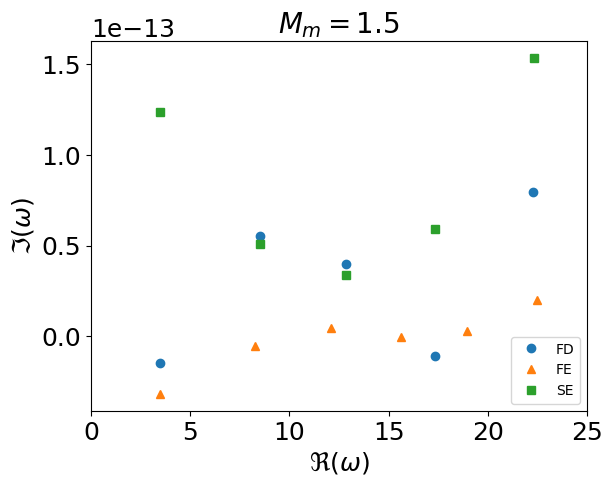
\includegraphics[width=0.7\linewidth]{../../thesis/img/numerical-experiments/fixed-fixed/supersonic-v}
	\caption{First few filtered eigenvalues are shown. The spurious modes are filtered by convergence test.}
	\label{fig:supersonic-v-dirichlet}
\end{figure}

\subsection{Fixed-Open Boundary}
\begin{figure} [H]
	\centering
	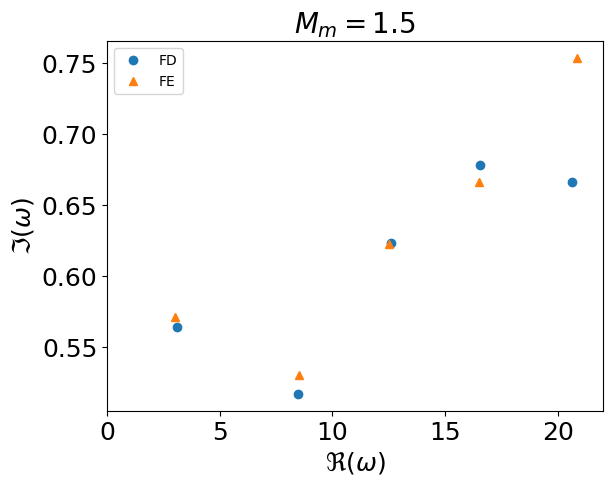
\includegraphics[width=0.7\linewidth]{../../thesis/img/numerical-experiments/fixed-open/supersonic-v}
	\caption{All modes are unstable.}
	\label{fig:supersonic-v-fixed-open}
\end{figure}


\section{Accelerating Case}
Starting from the singular point, we shoot the solution to the left boundary. We find the set of eigenvalues such that $\tilde{v}(-1)=0$. With these eigenvalues, we can extend the solution to the supersonic region $(0,1]$. The first five eigenvalues are drawn in the graph.
\begin{figure} [H]
	\centering
	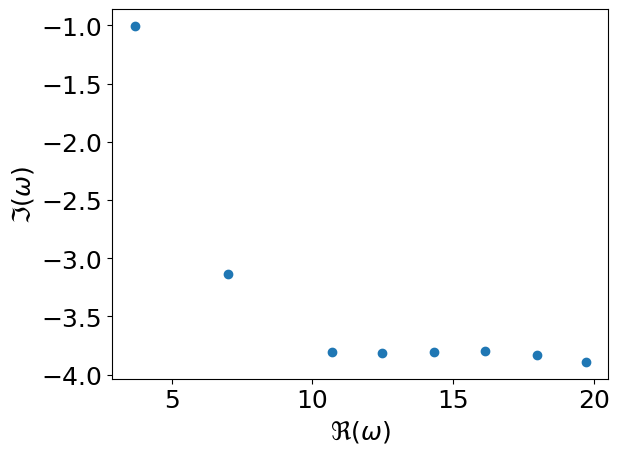
\includegraphics[width=0.7\linewidth]{../../thesis/img/numerical-experiments/accelerating-v}
	\caption{first five modes are stable.}
	\label{fig:accelerating-v}
\end{figure}
